\begin{table*}[t]
\centering\small
\begin{tabular}{llrrrr}
\toprule
Task & Tier & $B$ & Retrieval & Notes & Moderation \\
\midrule
SNACS & Luna & 0 & 40.1 (1) & shared B0 & shared B0 \\
SNACS & Luna & 4 & 37.6 (1) & 41.1 (1) & 40.1 (1) \\
SNACS & Luna & 16 & 43.6 (1) & 43.1 (1) & pending \\
SNACS & Luna & 64 & 45.5 (1) & 49.0 (1) & pending \\
SNACS & Sol & 0 & 71.3 (1) & shared B0 & shared B0 \\
SNACS & Sol & 4 & 71.8 (1) & 69.8 (1) & 70.8 (1) \\
SNACS & Sol & 16 & 67.8 (1) & 75.2 (1) & 71.8 (1) \\
SNACS & Sol & 64 & 76.7 (1) & 76.2 (1) & pending \\
CAP PA & Luna & 0 & 44.7 (1) & shared B0 & shared B0 \\
CAP PA & Luna & 4 & 32.6 (1) & 38.6 (1) & pending \\
CAP PA & Luna & 16 & 35.8 (1) & 31.6 (1) & pending \\
CAP PA & Luna & 64 & 41.9 (1) & pending & pending \\
CAP PA & Sol & 0 & 64.2 (1) & shared B0 & shared B0 \\
CAP PA & Sol & 4 & 64.7 (1) & 58.6 (1) & 61.9 (1) \\
CAP PA & Sol & 16 & 61.9 (1) & 65.6 (1) & 69.3 (1) \\
CAP PA & Sol & 64 & 65.1 (1) & 66.5 (1) & pending \\
\bottomrule
\end{tabular}
\caption{Observed primary accuracy (\%) and number of completed adaptation trajectories in parentheses. Pending cells have no imputed score. B0 is one shared retrieval starting point. Comparisons with incomplete or unequal trajectory counts are provisional. All evaluated targets, including refusals and call exhaustion, remain in denominators.}
\label{tab:subscription}
\end{table*}
At this snapshot, 32 of 112 configuration cells are complete. The transport ledger records 4,701 actor requests. Completed cell scores appear in Table~\ref{tab:subscription}; missing cells are not scored as zero. Operational statuses are retained separately from semantic errors.
No full three-seed paired condition contrast has completed in this snapshot; no adaptation-effect estimate is claimed.
\paragraph{Matched non-LLM controls.} All 45 control cells completed on the same new study samples and purchased trajectories. At $B=64$, mean primary accuracies over the three seeds are: snacs majority 13.4\%; snacs lexical majority 24.8\%; snacs tfidf nearest 15.7\%; cap pa majority 3.3\%; cap pa tfidf nearest 13.2\%. These controls do not receive guideline knowledge. They are diagnostics, not substitutes for a strong full-context model baseline.
\begin{figure*}[t]
\centering
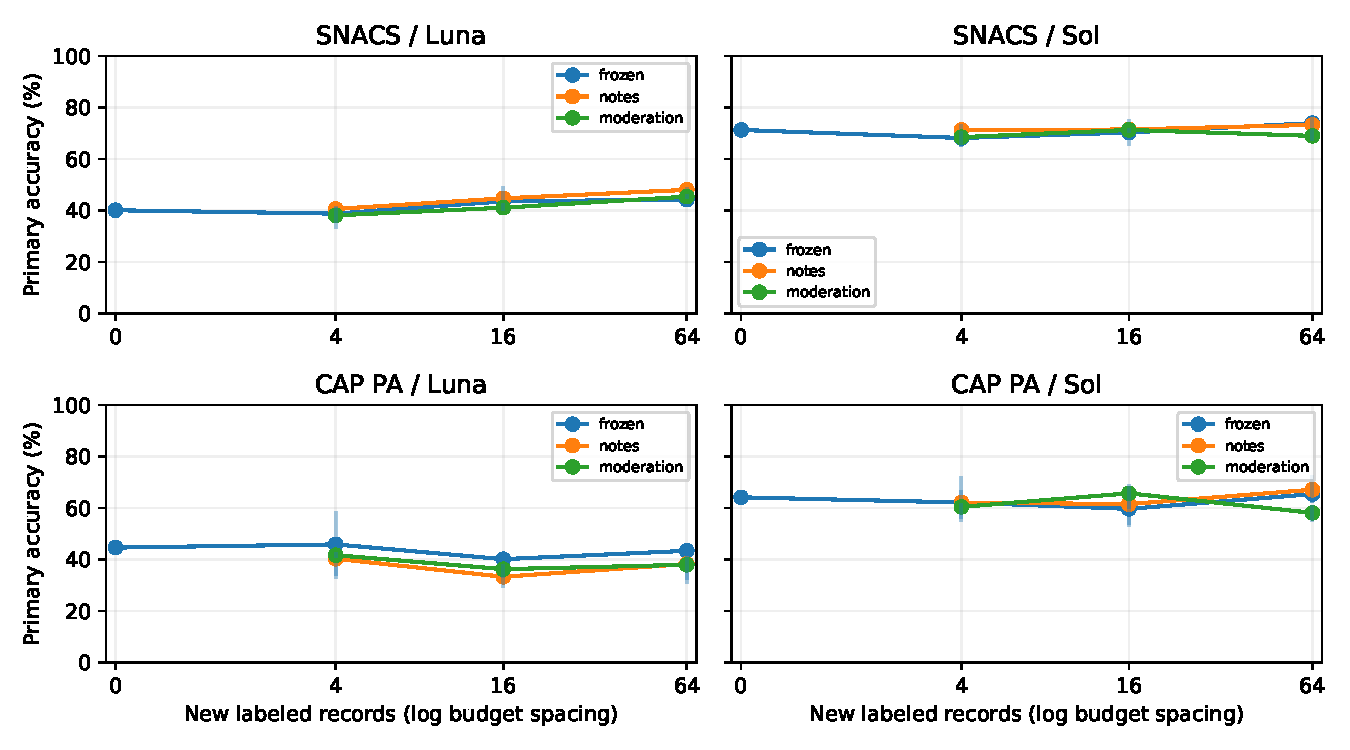
\includegraphics[width=.92\textwidth]{subscription-curves.pdf}
\caption{Observed completed-cell means. Vertical ranges span completed trajectory values, not confidence intervals; absent points are pending. The figure is descriptive until the planned trajectories complete.}
\end{figure*}
